\subsection{Dataset Creation}

Datasets were created to test the performance of the observability model and to evaluate the impact of \vbee{} on SLAM systems. We use both synthetic and real-world data to provide a diverse set of scenarios.

\subsection{Observability Scenario Dataset}
\label{sec:observability_scenario_dataset}

The Observability Scenario Dataset is a synthetic set of unique observability scenarios designed to evaluate the \knn{} model. Each scenario (a \textit{world}) is represented as a spherical volume with a single map point at the center. Worlds contain two barrier types: \textit{keep-out zones} and \textit{obstructions}. Keep-out zones represent viewpoints relative to the map point that the camera cannot access (e.g., below ground). Obstructions represent objects the camera can move behind that block observation of the map point (e.g., a wall to an adjacent room). A world specifies a barrier type for each of the six directions \(x^+, y^+, z^+, x^-, y^-, z^-\). Barriers can be placed either \textit{near} (touching the map point) or \textit{far} (at a distance of \(\dmax/2\) from the map point). For each direction, one of the following options is chosen:
\begin{itemize}
    \item (0) No obstruction
    \item (1) Near obstruction
    \item (2) Far obstruction
    \item (3) Near keep-out zone
    \item (4) Far keep-out zone
    \item (5) Near obstruction, far keep-out zone
\end{itemize}

A world is defined by a 6-tuple of barrier types \(b_{\text{direction}}\), representing the selection for each of the six directions:
\[
    world = (b_{x^+}, b_{y^+}, b_{z^+}, b_{x^-}, b_{y^-}, b_{z^-}).
\]
For example, the world \((0,0,0,0,0,0)\) represents free space, while \((1,0,0,0,0,0)\) represents a near obstruction in the \(x^+\) direction (e.g., a wall). This definition yields \(6^6 = 46{,}656\) worlds, although not all are valid or unique. Invalid worlds are those that would not allow the map point to be observed from any direction (e.g., two opposing near barriers). These can be eliminated by removing any worlds where \(world[i] \in \{1,3,5\} \land world[i+3]\in \{1,3,5\}\) for \(i \in \{0,1,2\}\). Next, reflections about the \(x,y,z\) axes and rotations that produce equivalent observability are removed. This results in 896 unique worlds used to evaluate the model.

This dataset enables controlled testing of viewpoint-dependent observability. Worlds can be queried to determine whether a map point is observable from a given viewpoint \(\viewpoint\), and the model can be evaluated based on its ability to predict the ground-truth observability. Figure \ref{fig:world_obs} shows an example world with two far obstructions and a far keep-out zone, queried with 1000 random viewpoints.

\begin{figure}[H]
    \centering
    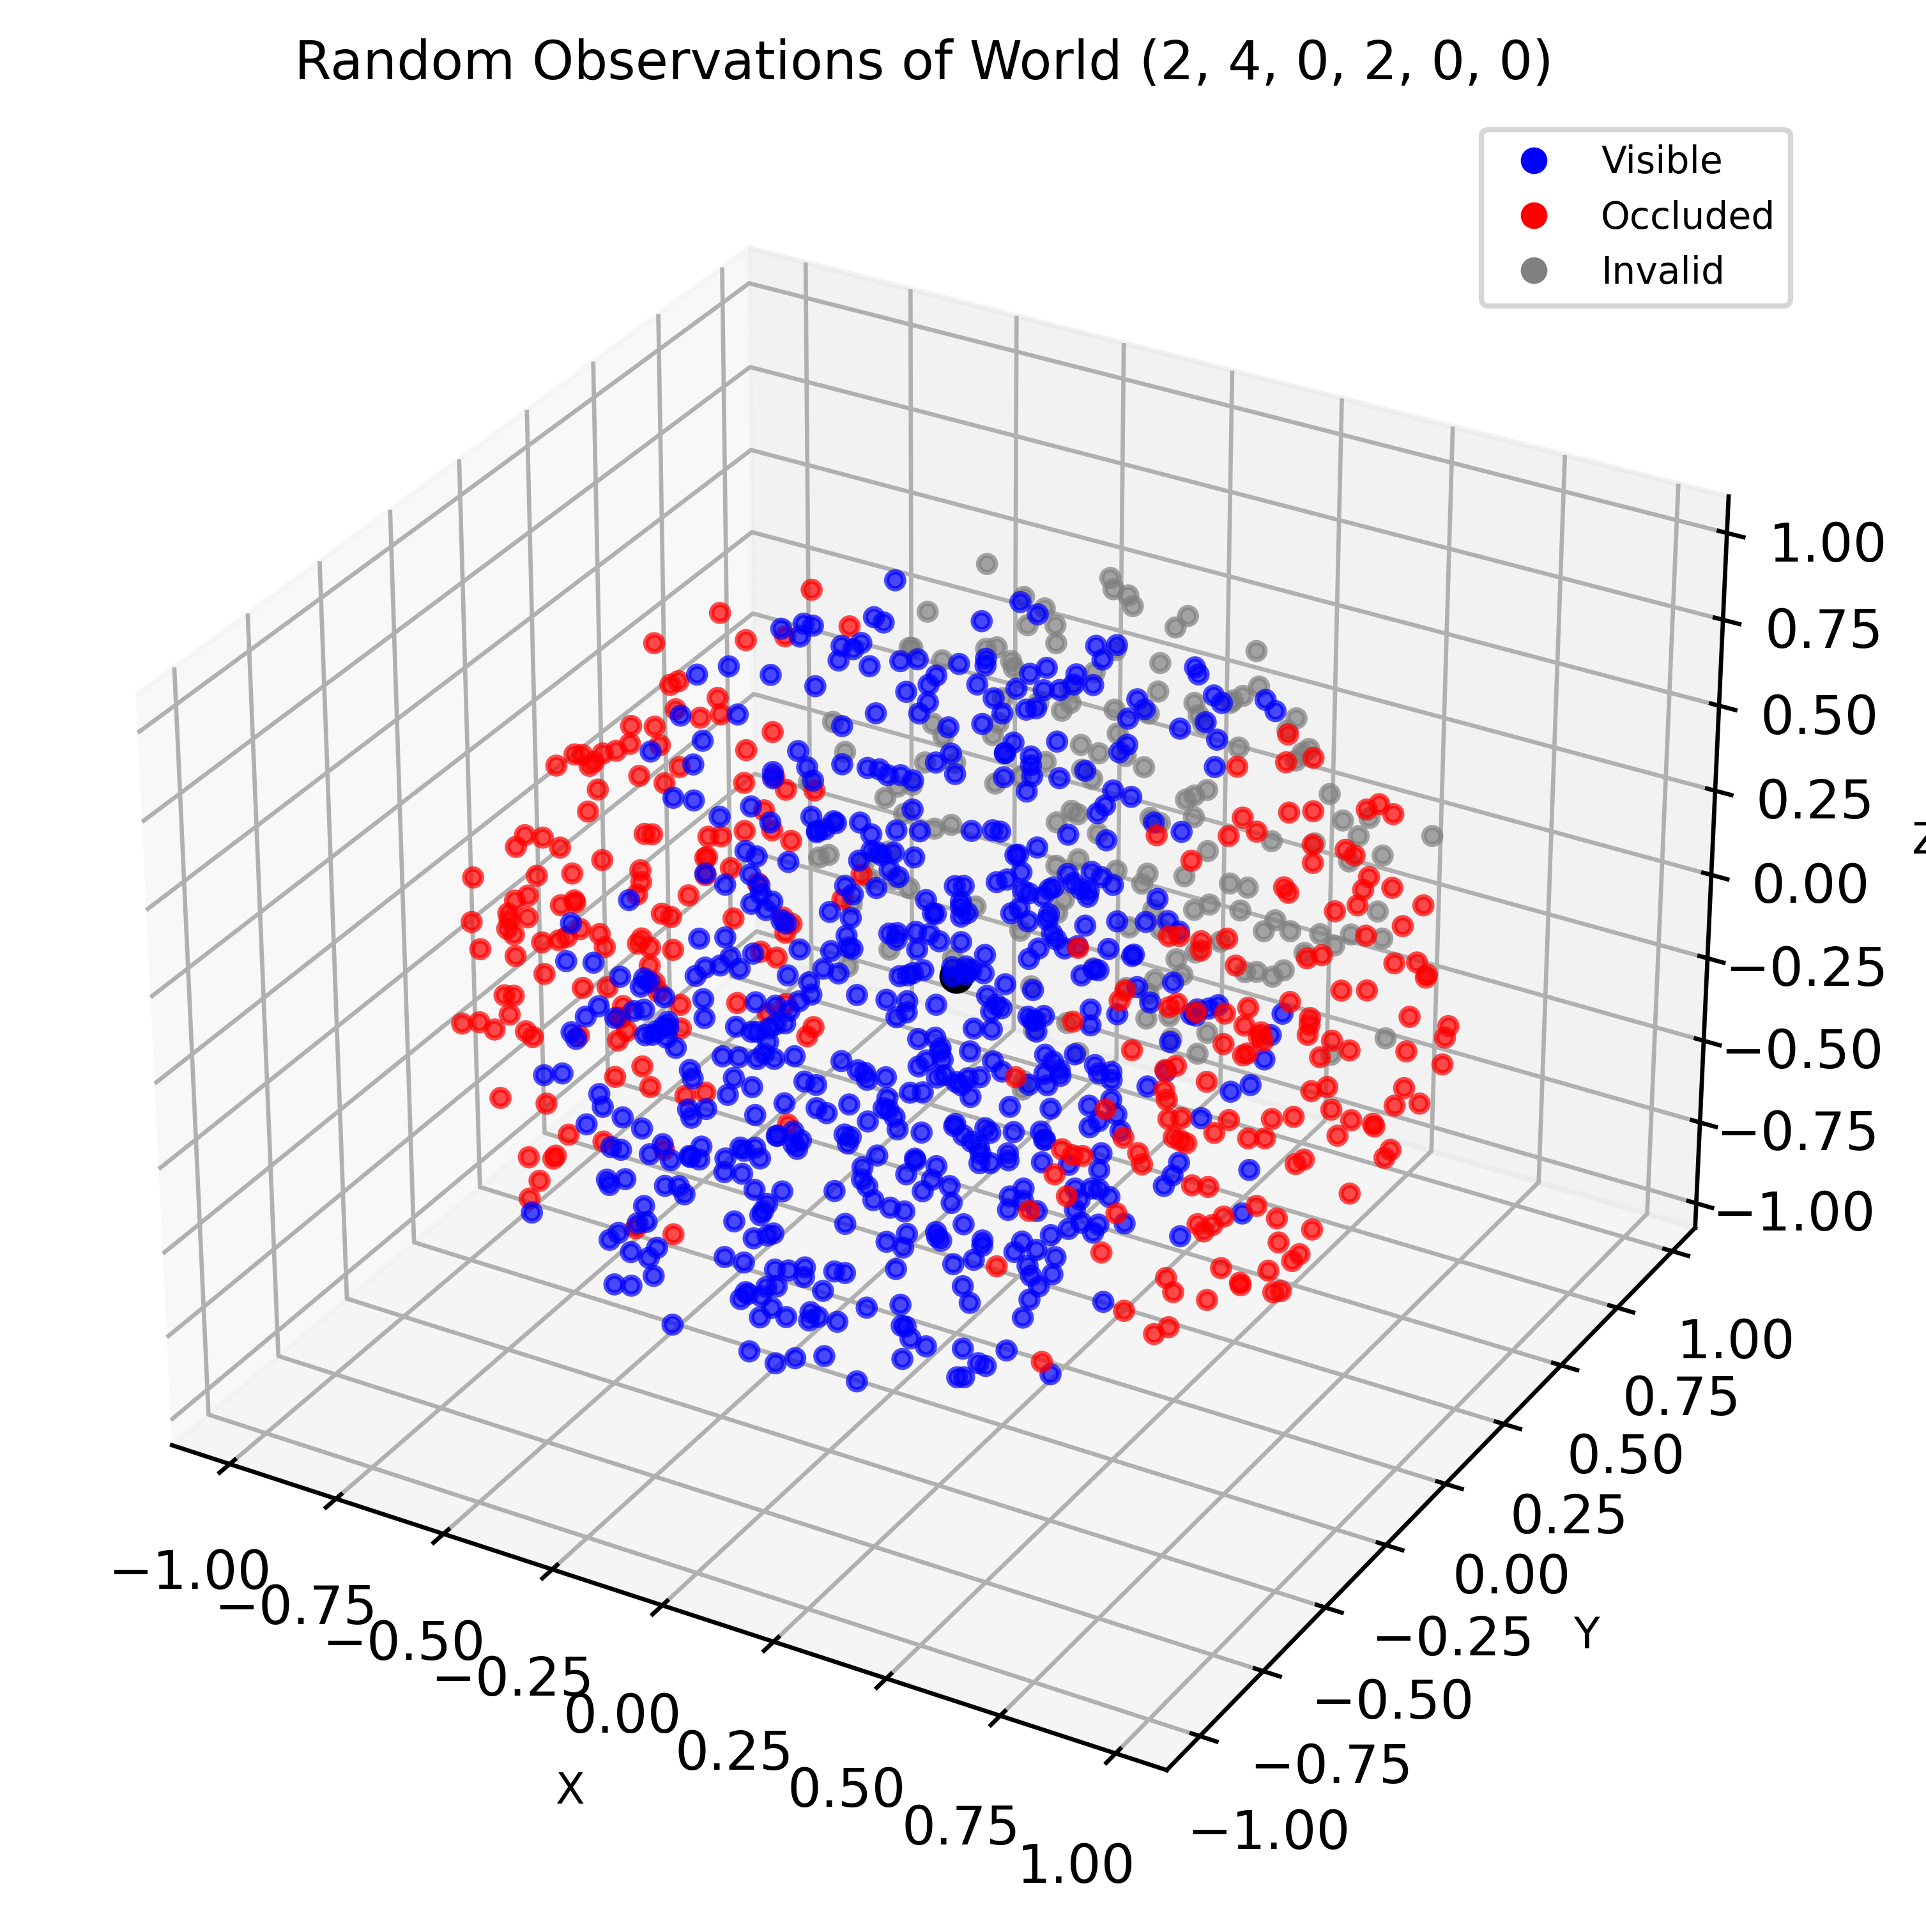
\includegraphics[width=0.8\textwidth]{resources/world_obs.png}
    \caption{1000 random viewpoints of world \((2, 4, 0, 2, 0, 0)\), showing the observability of the map point at the center.}
    \label{fig:world_obs}
\end{figure}

\subsubsection{Episodic Visual SLAM Dataset}

To evaluate \vbee{} in a real SLAM system, we created a stereo visual dataset consisting of trajectories through a household environment. No dynamic changes occur during individual trajectory recordings, but changes occur between recordings, matching the episodic modality discussed in Section \ref{sec:background}. Figure \ref{fig:episodic_datasets} shows example images from each trajectory at roughly the same location.

\begin{figure}[H]
    \centering
    
\includegraphics[width=0.8\textwidth]{resources/placeholder.jpeg}
    \caption{Example images from each trajectory of the Episodic Visual SLAM Dataset.}
    \label{fig:episodic_datasets}
\end{figure}

This dataset provides a realistic scenario for episodic KV-SLAM operation in a household environment. Because dense ground truth is difficult to obtain at scale, evaluation focuses on the SLAM system’s ability to maintain a consistent map across trajectories. \vbee{} is integrated into ORB-SLAM3, and performance is evaluated by its ability to perform MPR (removing outdated map points) while preserving a stable map across episodes.
